\documentclass{article}

\usepackage[english]{babel}
\usepackage[letterpaper,top=2cm,bottom=2cm,left=3cm,right=3cm,marginparwidth=1.75cm]{geometry}

\usepackage{amsmath}
\usepackage{graphicx}
\usepackage{float}
\usepackage[colorlinks=true, allcolors=blue]{hyperref}

\title{Calibration Tool - User Manual}
\author{Lovicourt Léo}

\begin{document}
\maketitle


\section{Available models}

\subsection{Perspective}

A perspective camera is designed to mimic the way the human eye sees. It is the most common projection mode used for rendering a 3D scene. It has several parameters available for estimation :

\begin{itemize}
    \item Focal length : distance from the camera's center to the image plane.
    \item Principal point : point at the intersection of the optical axis and the image plane.
    \item Distorsions : distorsions coefficients (k1, k2, k3 are the radial distorsion coefficients, and p1, p2 are the tangential distorsion coefficients). 
\end{itemize}

\begin{figure}[H]
\centering
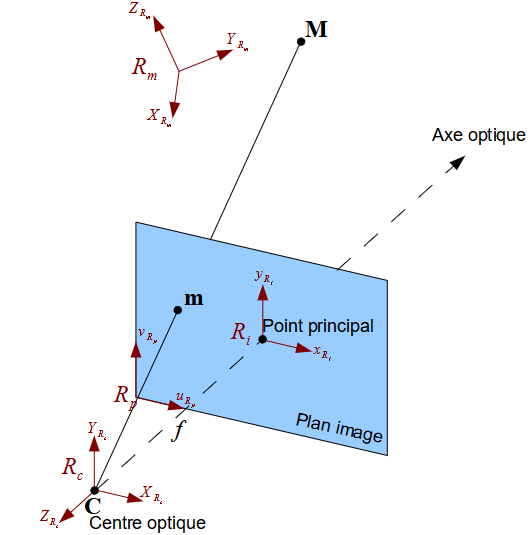
\includegraphics[width=0.7\textwidth]{stenope_schema.png}
\caption{\label{fig:stenope_schema}Schema of the model used for perspective cameras.}
\end{figure}

\newpage
\subsection{Spherical}

A spherical camera has a field of view that covers approximately an entire sphere, or at least a full circle in the horizontal plane.

\begin{itemize}
    \item Skew : number of pixels per unit length in each direction on the sensor. 
    \item Xi : parameter describing the mirror shape (Christopher Mei's model).
    \item Distorsions : distorsions coefficients (k1, k2 are the radial distorsion coefficients, and p1, p2 are the tangential distorsion coefficients). 
\end{itemize}

\begin{figure}[H]
\centering
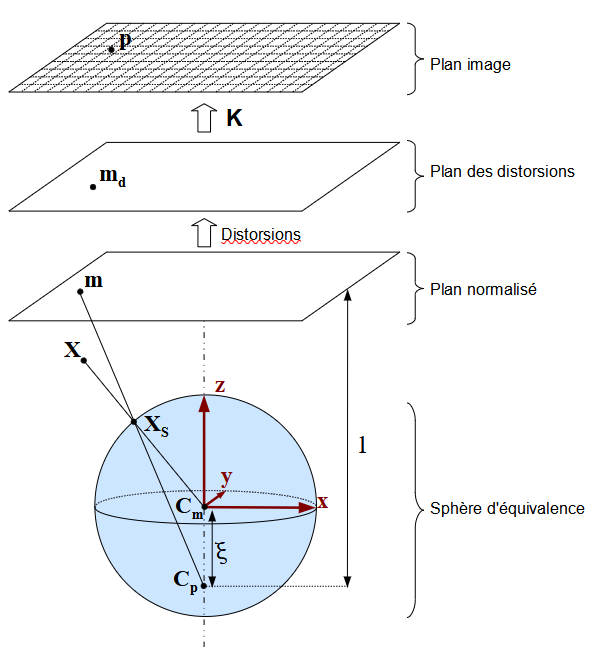
\includegraphics[width=0.7\textwidth]{omni_schema.png}
\caption{\label{fig:omni_schema}Schema of the model used for spherical cameras.}
\end{figure}

\section{Utilisation}

\subsection{Presentation of the user interface}

The user interface is fairly easy to use. At first, 4 buttons are displayed on the screen, each having a specific function.

\begin{itemize}
    \item \textbf{Perspective camera} - Allows a calibration on a perspective camera.
     \item \textbf{Spherical camera} - Allows a calibration on an omnidirectional camera.
     \item \textbf{About} - Displays a short help message with a button to access the program documentation (this file).
     \item \textbf{Exit} - Quits the program.
\end{itemize}



\begin{figure}[H]
\centering
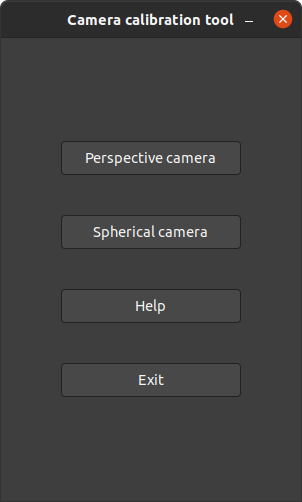
\includegraphics[width=0.3\textwidth]{main_menu.png}
\caption{\label{fig:main_menu}Main menu of the program.}
\end{figure}

To start any kind of calibration, the user must choose one of the two calibration types available.

\subsection{Load images}

To perform both calibrations, the user will have to provide at least 3 images of same dimensions. The file formats supported are \textit{.bmp, .tiff, .jpg, .pgm and .png}. Once images are chosen and if they are valid, they will be displayed as a mosaic.

\begin{figure}[H]
\centering
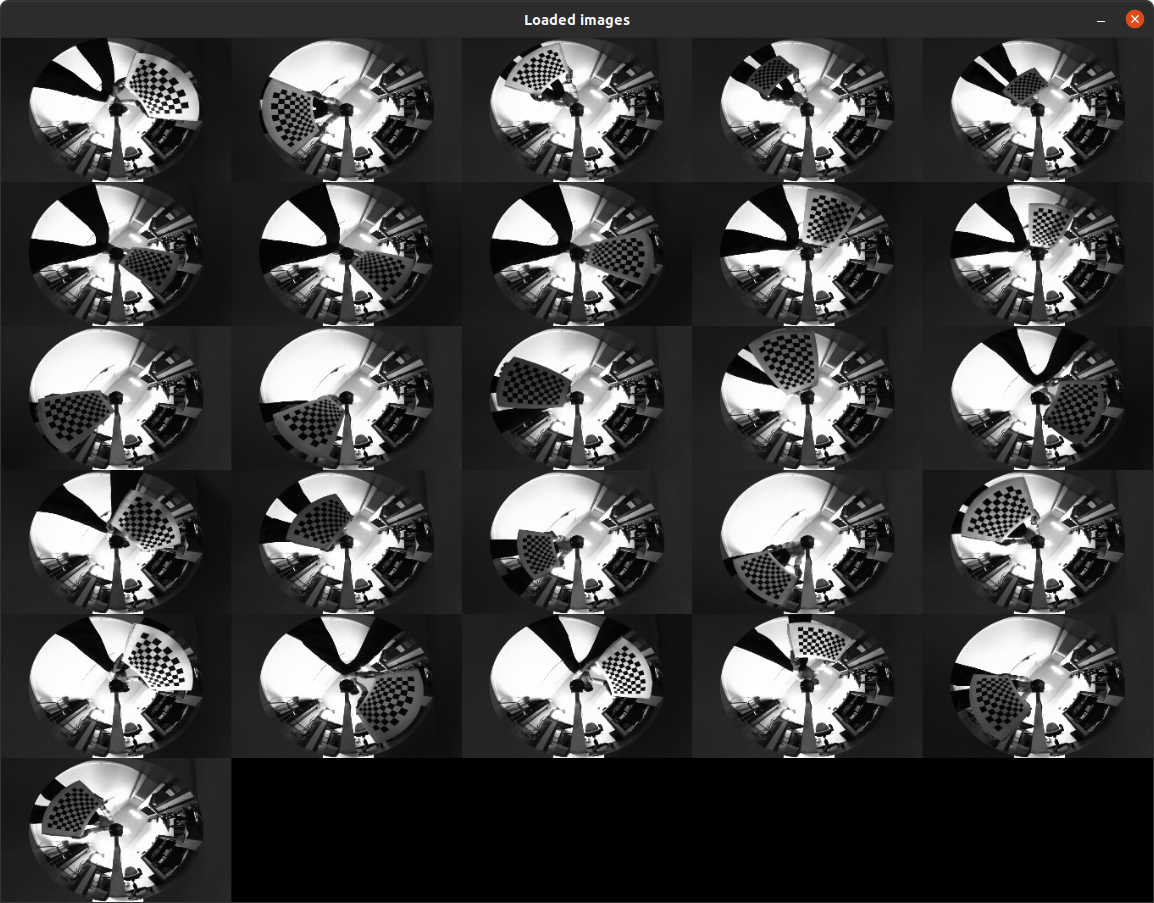
\includegraphics[width=0.8\textwidth]{mosaic.png}
\caption{\label{fig:mosaic}Mosaic containing images loaded.}
\end{figure}

\subsection{Extract grid corners}

This operation allows the user to extract the grid corners from each selected image.
All images will be displayed one by one in a window, and corners will have a red cross on them if the board was found. The board size must be at least $4\times 4$, and for a $n\times m$ grid, there should be $(n - 1)\times (m - 1)$ corners found.
The user will have multiple ways to go through all selected images.
\begin{itemize}
    \item \textbf{Pressing Enter, Y, or O} to set this image as valid and go to the next image.
    \item \textbf{Pressing N} to specify that this image shouldn't be used for calibration and go to the next image.
\end{itemize}

The user also has the possibility to zoom on an image. To do so, he has to hold the \textbf{left-click} on the image and draw a rectangle around the desired area. Once the selection is done, press \textbf{Enter} to confirm selection and perform a zoom, or press \textbf{Escape} to undo the selection. A \textbf{left-click} on the image will have the same effect as pressing Escape.
Once a zoom has been performed, the user can return to the initial view by pressing \textbf{Escape}, or go to to the next image using the keys presented earlier.\bigskip

A valid image is one whose corners have all been detected and colored.\bigskip

\textit{Note : the program will itself set an image as not valid if not any corner has been found.}\bigskip

\begin{figure}[H]
\centering
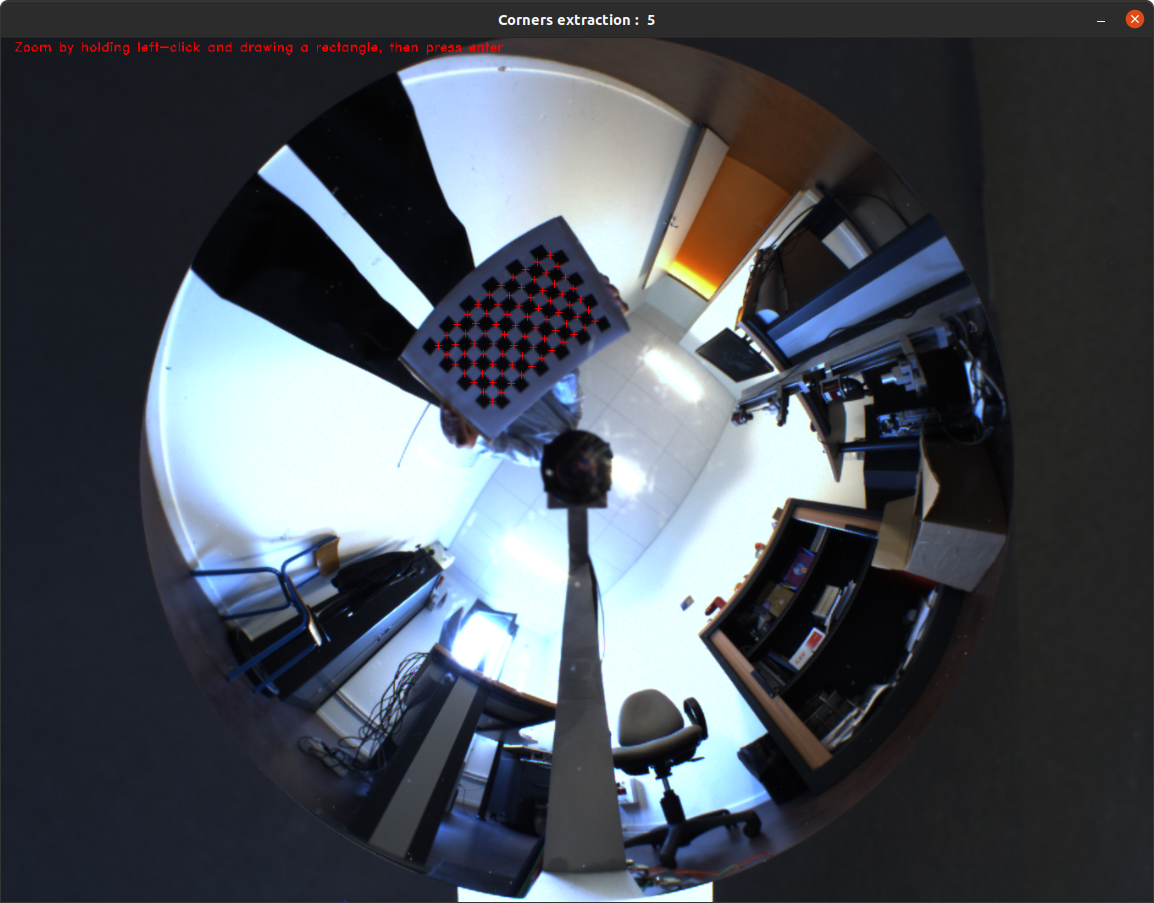
\includegraphics[width=0.8\textwidth]{egc.png}
\caption{\label{fig:egc}Corners extraction of an image.}
\end{figure}

After going through all the images, a popup will ask the user if the extraction was successful. The user can select \textbf{"No"} to do another extraction with eventually other parameters and other images, or \textbf{"Yes"} to then perform calibration.

\subsection{Calibration}

As the program has now all the required data, the user can now perform calibration. Once the operation is done, a popup will appear to tell the user the calibration was successful. However, it may fail if the user has set images as valid even though they are not.

\subsection{Show corners reprojection}

By clicking on this button, the user will go again through all the \textbf{valid} images to view the reprojection of the corners calculated for each frame. For each corner, it will have a green cross displayed were the corner was found during extraction, and a red cross at the recalculated position of this corner. There will finally be a legend at the bottom-left of the image, including these two crosses and the error rate (in pixel) of the image.

\begin{figure}[H]
\centering
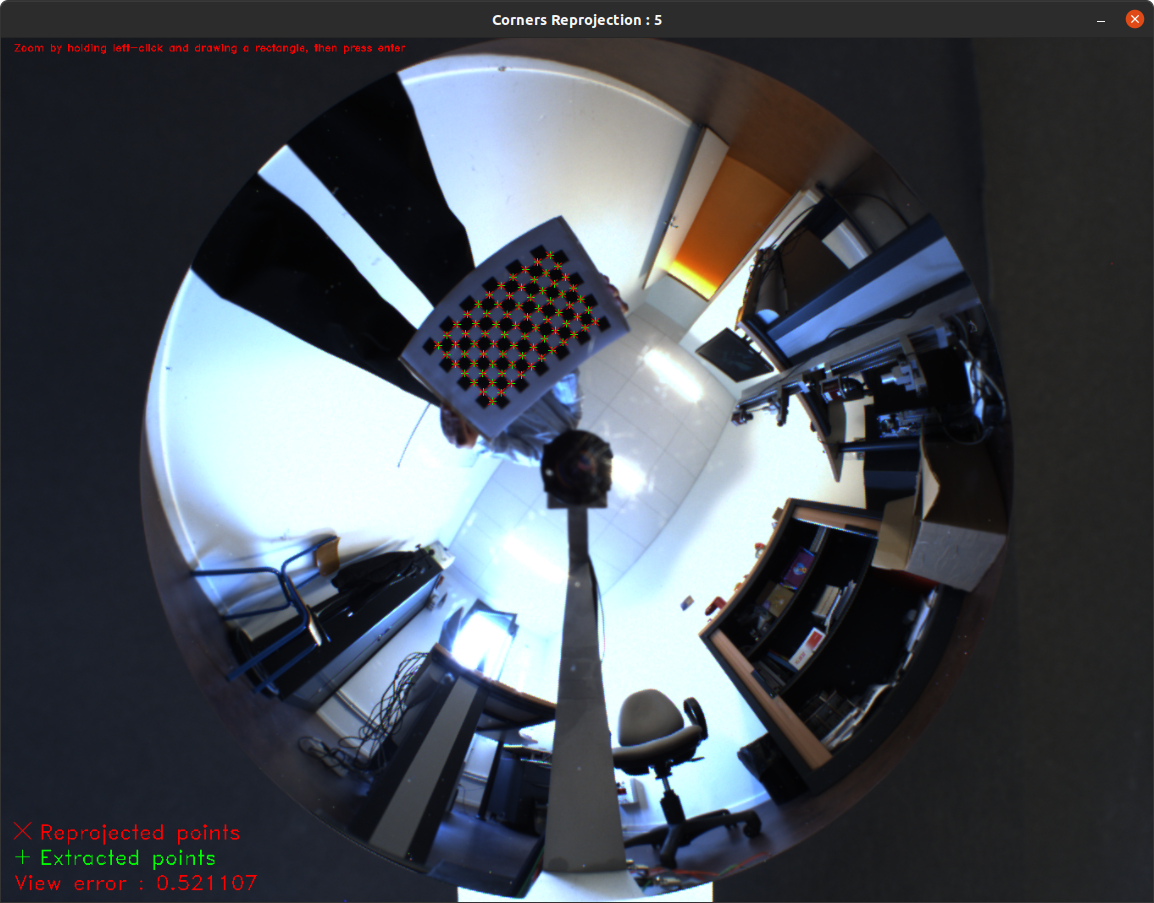
\includegraphics[width=0.9\textwidth]{sr.png}
\caption{\label{fig:sr}Corners reprojection of an image after calibration.}
\end{figure}

\subsection{Calibration results}

A frame will appear on the screen, with the results of the calibration. It will contain various informations, depending on the type of calibration performed, but also the informations about the images used for calibration.

\begin{figure}[H]
\centering
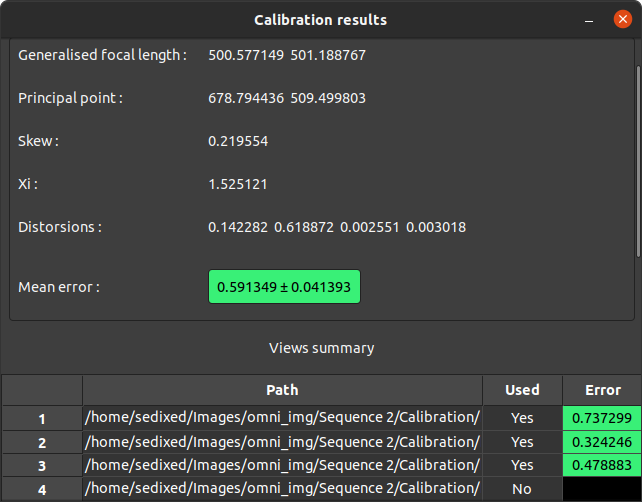
\includegraphics[width=0.8\textwidth]{results.png}
\caption{\label{fig:results}Spherical calibration results.}
\end{figure}

\subsection{Save}

The user can save the results of the calibration after clicking on \textbf{"Calibration results"} as an YML file. It will contain all the data calculated through the calibration, and more precisely :
\begin{itemize}
    \item Type of calibration performed (perspective / spherical)
    \item Number of images provided
    \item Properties of the mire used
    \item Mean error
    \item Method used \textit{(Perspective only)}
    \item Render size and search size
    \item Intrinsics parameters
    \item Distorsions coefficients
    \item Skew \textit{(Spherical only)}
    \item Flags (integer form)
    \item Images data (validity, path, error rate, extrinsics parameters)
\end{itemize}

\subsection{Load YML file}

The user can load a YML file previously saved through this program. By doing so, it will set all the parameters according to the values readed in the file chosen.
However, this operation may fail if the file has been modified externally with incorrect data.

\subsection{Preferences}

The user can set some preferences for the calibration. Except the parameters to estimate that have to be selected before calibration, they have to be selected before grid corners extraction, otherwise the user will have to extract the corners again.\newline
A parameter is fixed if its checkbox is unchecked, otherwise it will be estimated by the program.

\begin{itemize}
    \item \textbf{Parameters to estimate} : these are parameters the user can choose to fix to a default value that will be used for calibration.
    
    \begin{enumerate}
        \item \textbf{Focal length} \textit{(Perspective only)} : can be fixed using two values.
        \item \textbf{Principal point} : can be fixed to the center of an image loaded.
        \item \textbf{Distorsions} : each of the distorsion coefficients can be fixed to 0.
        \item \textbf{Method} \textit{(Perspective only)} : the frame provides a button to select the calibration method used. The \textbf{RO} (\textbf{R}eleasing \textbf{O}bjects) method is an extension of the default one. In many common cases with inaccurate, unmeasured, roughly planar targets (calibration plates), this method can dramatically improve the precision of the estimated camera parameters.
        \item \textbf{Skew} \textit{(Spherical only)} : can be fixed to 0.
        \item \textbf{Xi} \textit{(Spherical only)} : can be fixed to 1.
    \end{enumerate}
    
    \item \textbf{Size of the window for the corners detection} : When the corners are being extracted, an automatic procedure is used to refine its coordinates. The size of the window used can be specified here.
    
    \item \textbf{Render window size} : Preferred size of the window in which the images are displayed.
    
    \item \textbf{Calibration pattern properties} : The pattern properties are very important to obtain
    good results. The size of the squares has to be set according to the pattern you are using. All
    measurements are in millimeters.
\end{itemize}

\begin{figure}[H]
\centering
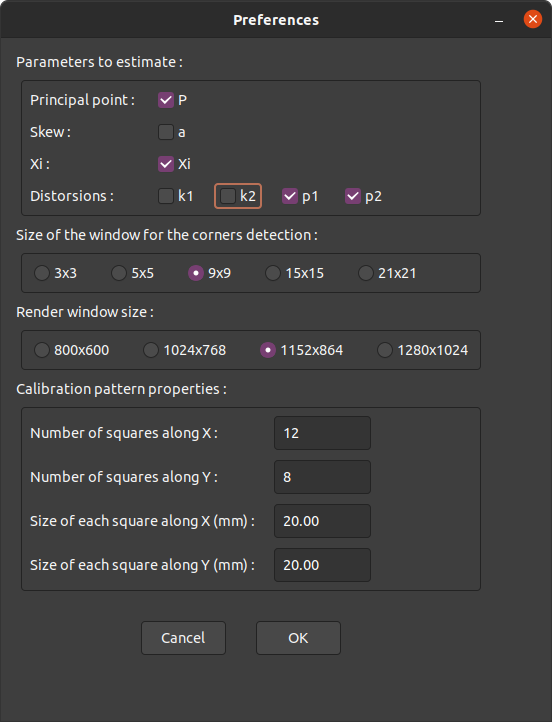
\includegraphics[width=0.6\textwidth]{pref.png}
\caption{\label{fig:pref}Preferences frame for a spherical calibration.}
\end{figure}

\textit{Note : the parameters to estimate won't be editable before loading images as it requires the size of an image for the principal point.}


\subsection{Exit}

Quits the program.

\end{document}